\section{Operations with transfer functions}

Let $W(z)$ and $M(z)$ denote the transfer functions of linear digital filters.

\paragraph*{Series connection}
When connecting these transfer functions in series, the resulting block diagram is as follows:
\begin{figure}[H]
    \centering
    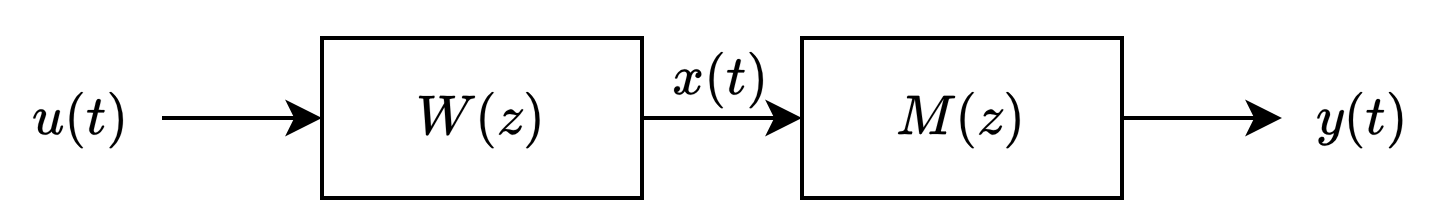
\includegraphics[width=0.75\linewidth]{images/series.png}
\end{figure}
This configuration yields the following equations:
\[\begin{cases}
    y(t)=M(z)x(t) \\
    x(t)=W(z)u(t)
\end{cases}\]
By substitution, we obtain:
\begin{align*}
    y(t)    &=M(z)\left[ W(z)u(t) \right] \\G
            &=M(z)W(z)u(t) \\
            &=V(z)u(t) \\
\end{align*}
Hence, the transfer function of $n$ blocks in series is the product of the transfer functions of each block.

\paragraph*{Parallel connection}
When connecting the transfer functions in parallel, the block diagram appears as follows:
\begin{figure}[H]
    \centering
    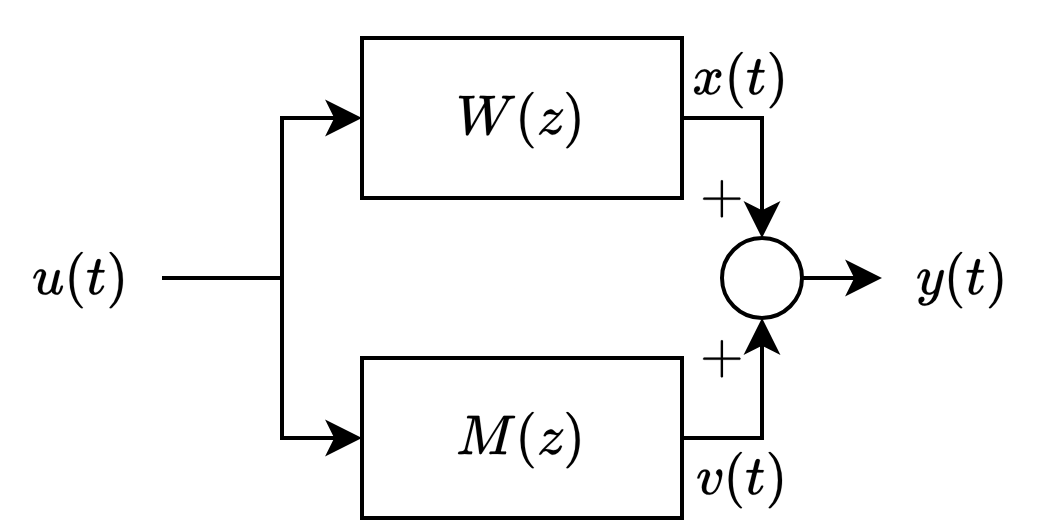
\includegraphics[width=0.5\linewidth]{images/parallel.png}
\end{figure}
The output signal is the sum of the two signals:
\begin{align*}
    y(t)    &=x(t)+v(t) \\
            &=W(z)u(t)+M(z)u(t) \\
            &=\left(W(z)+M(z)\right)u(t) \\
            &=V(z)u(t)
\end{align*}
Consequently, the transfer function of $n$ blocks in parallel is the sum of the transfer functions of each block.